%! Author = jannikeschler
%! Date = 18/09/2022

\documentclass[reprint,english,notitlepage]{revtex4-2}
\usepackage{amsmath}
\usepackage[mathletters]{ucs}
\usepackage[utf8x]{inputenc}
\usepackage[english]{babel}
\usepackage{esint}
\usepackage{physics,amssymb}
\usepackage{graphicx}
\usepackage{xcolor}
\usepackage{hyperref}
\usepackage{listings}
\usepackage{subfigure}
\hypersetup{
    colorlinks,
    linkcolor={red!50!black},
    citecolor={blue!50!black},
    urlcolor={blue!80!black}}

\lstset{inputpath=,
	backgroundcolor=\color{white!88!black},
	basicstyle={\ttfamily\scriptsize},
	commentstyle=\color{magenta},
	language=Python,
	morekeywords={True,False},
	tabsize=4,
	stringstyle=\color{green!55!black},
	frame=single,
	keywordstyle=\color{blue},
	showstringspaces=false,
	columns=fullflexible,
	keepspaces=true}

\begin{document}
\title{Simulating Planetary orbits of a solar system}
\author{Jannik Eschler \& Oskar Idland}
\date{\today}
\affiliation{Institute of Theoretical Astrophysics, University of Oslo}

\begin{abstract}
This is an abstract \colorbox{red}{Complete this summary at the end of the paper}
\end{abstract}
\maketitle

\section{Introduction}
When making our way out of the earth's atmosphere, we will have to know where our destination will be after the launch.
To be able to reach our destination we therefore have to get known in our solar system and explore and simulate the different planets in the system.
After finding out the orbits of the planets, it will be much easier to coordinate our launch to our target to minimize the time and effort required to find the destination.
Using this, we will also be able to give estimates about the possibility of extraterrestrial life discovering our solar system.

\section{Method}
The calculation of the planetary orbits in our solar system can either be done numerically or analytically.
Both methods have their advantages and disadvantages compared to the other.
To be able to find the analytical orbit of a planet, we will first have to find an analytical expression for the orbit of a planet.
As planetary orbits usually are ellipses with the star positioned in one of the two foci of the ellipse, we will be able to derive a formula for the position of the planet based on the formula for and ellipse.
An ellipse is defined as "A closed plane curve generated by a point moving in such a way that the sums of its distances from two fixed points is a constant." \colorbox{red}{Merriam Webster}
The analytical expression for an ellipse in cartesian coordinates with the origin in the middle is given by
\begin{align}
    \frac{x^2}{a^2} + \frac{y^2}{b^2} = 1 \label{ellipse_analytic_cart}
\end{align}
For the calculations in this report, it is however advantageous to be able to use this expression in polar coordinates.
When switching to polar coordinates, we will be using the distance $r = |\textbf{r}|$ from the star in one focus point to the point on the ellipse and the angle $f$ at the star from the semi-major axis to the vector $\bold{r}$ as seen in figure \ref{fig:Ellipse_fig}.
In orbital mechanics, the angle $f$ is also often called the true anomaly.
\begin{figure}[h]
	%% h(here), t(top of page), b(bottom of page)
	\centering
	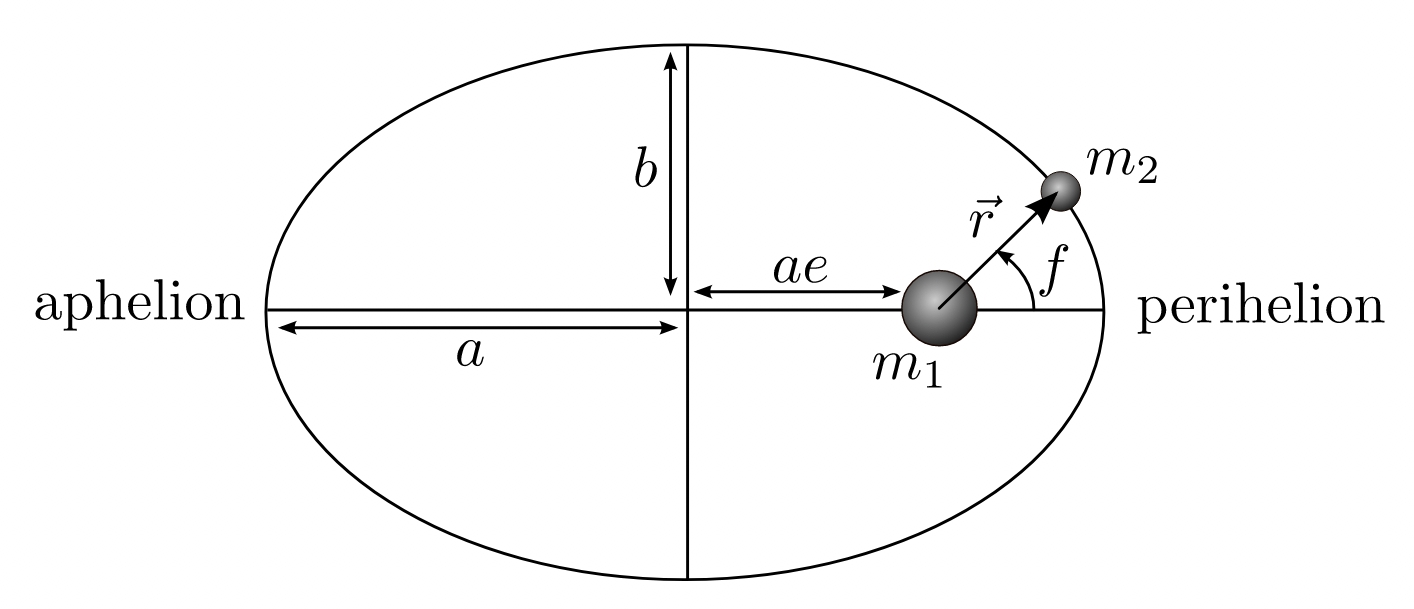
\includegraphics[scale=0.3]{Figures/Ellipse}
	\caption{Figure of an ellipse with all major components}\label{fig:Ellipse_fig}
\end{figure}
Based on figure~\ref{fig:Ellipse_fig} we are now able to see that
\begin{align}
    &x = ae + r\,cos(f) \label{x_ellipse}\\
	&y = r\,sin(f) \label{y_ellipse}
\end{align}
Using equations~\ref{x_ellipse} and~\ref{y_ellipse} we wre now able to find an equation for the distance $r$
\begin{align*}
    r = \frac{a(1-e^2)}{1 + e\,cos(f)}
\end{align*}
with e being the eccentricity of the ellipse given by 
\begin{align*}
    e = \sqrt{1-\frac{b^2}{a^2}}
\end{align*}
Here, a is the semi-major axis and b is the semi-minor axis of the ellipse.
Now, $r$ can be used to convert the coordinates back to cartesian coordinates using equations~\ref{x_ellipse} and~\ref{y_ellipse}.
By iterating over a collection of equally spaced values between $0$ and $2\pi$, we will find collection of points on the elliptical orbit of the planets, which can then be plotted.
When repeating this for each planet using the given constants for each planet, we will be able to simulate the orbits or all planets.\\\\
The analytical expression, can be used to find the orbit of a given planet, but not the velocity or the position of the planet on the orbit the planet at a given time.
To find the position of the planet in the orbit as a function of time, we will first need to simulate the orbit numerically.
The general idea of the simulation is to use newtons second law $\sum\bold{F} = m\bold{a}$ to calculate the acceleration of the planet at a certain position.
In this simulation, all forces except gravitational forces from the star will be neglected.
Therefore the total force exerted on the planet can be calculated using Newtons law of universal gravitation.
\begin{align*}
    &\sum\bold{F} = G\,\frac{m_1 m_2}{r^2} \label{Newton_Grav_law}\\
	&\sum\bold{F} = m_1 \bold{a}\\
	&\bold{a} = G\,\frac{m_1}{r^2}
\end{align*}
With $G$ being the gravitational constant, $m_1$ being the mass of the star, $m_2$ being the mass of the planet, and $r$ being the distance between the star and the planet.\\\\
Using the initial velocity of the object at the position we are calculating the acceleration for, as well as the acceleration, we can find the velocity after a small time interval $\Delta t$.
Correspondingly, using the initial position and velocity, the position after the time step $\Delta t$ can be calculated.
The process is then repeated using the new position and velocity to calculate the acceleration in the point and velocity and position after another time interval $\Delta t$.
There are different variations of this process, with different advantages and disadvantages.\\
In this simulation the Leapfrog method will be used.
This method calculates the acceleration in a point and uses it to find the velocity $\bold{v}_h$ after $ \frac{dt}{2}$.
Velocity $\bold{v}_h$ and the initial position of the planet will then be used to calculate the new position after a time interval $\Delta t$.\\
\begin{figure}[h]
	%% h(here), t(top of page), b(bottom of page)
	\centering
	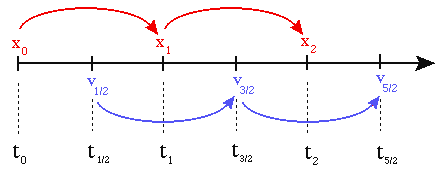
\includegraphics[scale=0.4]{Figures/leapfrog1}
	\caption{\colorbox{red}{Visualisation of the Leapfrog integration algorithm}}\label{fig:Leapfrog_vis}
\end{figure}\\
As $\bold{v}_h$ is somewhere between the velocity of the object in the initial position and the position after a time interval $\Delta t$, the calculation of the new position will be more exact.
The process can be described using three equations:
\begin{align*}
    \textbf{a}_i &= A(\textbf{x}_i)\\
	\textbf{v}_{i+1/2} &= \textbf{v}_{i-1/2} + \textbf{a}_i\,\Delta t\\
	\textbf{x}_{i} &= \textbf{x}_i + \textbf{v}_{i+1/2}\,\Delta t
\end{align*}
After simulating the orbits of the planets, the results can be used to find a function of time approximating the orbit of each planet.
This will be done by interpolating the results into a function.\\\\

To describe the orbits further, we can make use of Johannes Kepler's laws of planetary motion.
The three laws state:
\begin{enumerate}
    \item The orbit of a planet is an ellipse with the
		Sun in one of the foci.
	\item A line connecting the Sun and the planet
		sweeps out equal areas in equal time inter-
		vals.
	\item The orbital period around the Sun and the
		semimajor axis of the ellipse are related through:
		\begin{align*}
		    P^2 = a^3
		\end{align*}
		\colorbox{red}{where P is the period in years and a is the
		semimajor axis in Astronomic Units}
\end{enumerate}

To find out whether our results agree with Kepler's laws, a formula for calculating the area swept out by the vector $ \textbf{r}$ during a given time interval has to be found first.



\section{Results}
This section is for results only
	\subsection{Subsection}
    Subsection?

\section{Discussion}
To get an accurate simulation, the time interval dt need to be sufficiently small.
An adequate number is approximately 10'000 steps per year of simulation, which corresponds to a time interval of $\Delta t = 52$ min $33.6$ sec.
Using smaller time intervals will result in a more precise simulation, but will increase computing time.
	\subsection{Subsection}

\section{Conclusion}
And the conclusion


\section{References}
References are important!\\
1:\:https://www.merriam-webster.com/dictionary/ellipse\\
2:\:https://cvarin.github.io/CSci-Survival-Guide/leapfrog.html\\
3:\:https://www.uio.no/studier/emner/matnat/astro/AST2000/h22/undervisningsmateriell/lecture_notes/part1b.pdf

\section{Appendix: Mathematical Derivations}
	\subsection{Section 1}
	\begin{align*}

	\end{align*}

\end{document}